\textbf{Atenção:Os cálculos foram feitos com aproximações e condições de contorno especificadas ao 
decorrer do texto. Se usou uma situação ideal geral, sem embasamento em transferencia de calor ou 
matéria.Foi feito apenas para estimar a capacidade de produção de água.}

Para a determinação da a temperatura e umidade do ar de saída, utilizaremos as equações abaixo 
para determinar, numa aproximação razoável, quantidade de água que retiraremos do ar.   

A umidade relativa do ar é a porcentagem da quantidade máxima de água que o ar (nas mesmas 
condições de pressão e temperatura) consegue carregar\footnotemark.
Para determinar a quantidade de água no ar, usamos a equação:\footnotemark
\footnotetext{Disponível em: <http://www.azosensors.com/Article.aspx{?}ArticleID{=}23>. Acesso em 10/06/15}
\footnotetext{Disponível em: <http://glossary.ametsoc.org/wiki/Mixing\_ratio>. Acesso em 22/06/15}

\begin{equation}
 r = \frac{0.622e}{p - e}
\end{equation}[1]

Onde: O ar é considerado um gás perfeito constituído apenas de N,O e Ar.\\
r = razão de massa entre água e ar;\\
e = pressão parcial do vapor de água;\\
p = pressão atmosférica.

Para obtermos a quantidade de água presente no ar, precisamos da pressão atmosférica e da 
pressão parcial do vapor de água. A pressão atmosférica utilizada foi a pressão a 600m de altitude : 706 mmHg\footnotemark. A pressão de vapor da água, foi obtida pela junção da segunda e terceira equação da imagem 
abaixo, adotando os coeficientes da água entre 0 e 100 graus, retirados da tabela\footnotemark.
\footnotetext{Disponível em: <http://www.azosensors.com/Article.aspx{?}ArticleID{=}23>. Acesso em 10/06/15}
\footnotetext{Disponívek em: <http://www.engineeringtoolbox.com/airaltitudedensityvolume\_
195.html> Acesso 22/06/15}
\begin{figure}[!h]
    \centering
    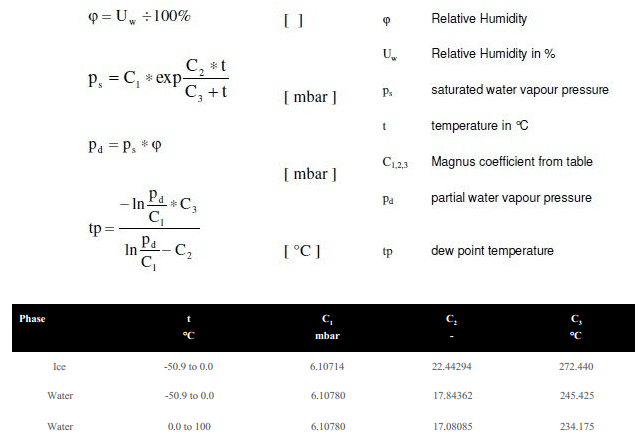
\includegraphics[scale = 1]{editaveis/figuras/tabela_calculo}
    \label{dados_agua}
    \caption[Propriedades físicas da água]{Propriedades físicas da água}
   \end{figure}
   \FloatBarrier
   
Chegamos então ao resultado de:
\begin{figure}[!h]
    \centering
    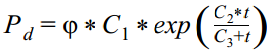
\includegraphics[scale = 1]{editaveis/figuras/eq_1calculo}
    \label{eq1_calculo}
    \caption[Equação Pd]{[2]}
   \end{figure}
   \FloatBarrier
Substituindo a $P_d$ da equação [2] em [1], e substituindo os valores de pressão atmosférica e das d
constantes, temos:
\begin{figure}[!h]
    \centering
    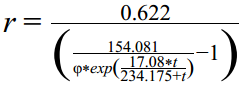
\includegraphics[scale = 1]{editaveis/figuras/razao_volumetrica}
    \label{dados_agua}
    \caption[Razão Volumétrica]{[3]}
   \end{figure}
   \FloatBarrier
Como r é a razão volumétrica, chegamos à expressão de fluxo de massa de água em função do
fluxo de massa de ar, umidade relativa e temperatura:
\begin{figure}[!h]
    \centering
    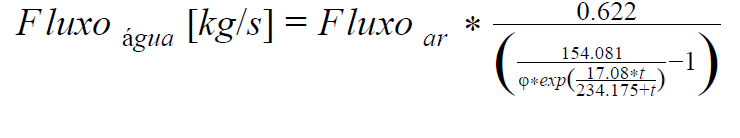
\includegraphics[scale = 0.6]{editaveis/figuras/fluxo_agua}
    \label{fluxo_agua}
    \caption[Fluxo água]{[4]}
   \end{figure}
   \FloatBarrier
Segundo o Serviço geológico do Brasil\footnotemark, Temos que a temperatura média anual de acarí é 29.6
graus celsius e a umidade média anual de 64%.
Resolvendo a equação [4] para esses dados, conseguimos o fluxo de água que entra variando apenas com
o fluxo de ar:
\footnotetext{Disponível em: <http://www.cprm.gov.br/rehi/atlas/rgnorte/relatorios/ACAR001.PDF > Acesso em: 10/06/15}
\begin{figure}[!h]
    \centering
    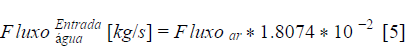
\includegraphics[scale = 1]{editaveis/figuras/fluxo_entrada}
    \label{fluxo_entrada}
    \caption[Fluxo entrada de água]{[5]}
   \end{figure}
   \FloatBarrier
 
Como a água não desaparece do sistema, Podemos afirmar que a diferença entre as massas de água da entrada e saída nos darão a água coletada.
\begin{figure}[!h]
    \centering
    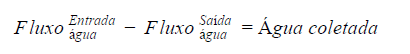
\includegraphics[scale = 1]{editaveis/figuras/diferenca}
    \label{diferenca_massa}
    \caption[Diferença entre as massas de água]{[6]}
   \end{figure}
   \FloatBarrier
Substituindo, temos
\begin{figure}[!h]
    \centering
    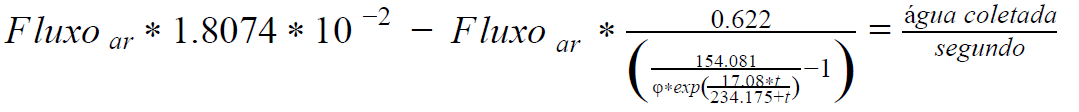
\includegraphics[scale = 0.6]{editaveis/figuras/fluxo_ar}
    \label{fluxo_ar}
    \caption[Diferença entre as massas de água]{[7]}
   \end{figure}
   \FloatBarrier
Como nosso evaporador foi preparado para 20 graus celsius e cerca de 3.6 kg de ar por segundo,
esses serão os valores de temperatura de saída e fluxo de ar..Considerando o pior dos casos dessa
desumidificação, a ar sairía saturado, ou com umidade relativa de 100\%. Usando esses valores,
temos:
\begin{figure}[!h]
    \centering
    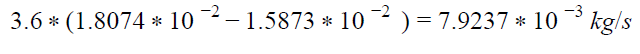
\includegraphics[scale = 1]{editaveis/figuras/calculo}
    \label{calculo_final}
    \caption[Calculo Final]{[7]}
   \end{figure}
   \FloatBarrier
Convertendo-se para kg/dia, temos: 684,61 kg/dia.